%% skeleton.tex                 %% 12 February 2006
%% Use this file to start your paper for the UJM/18.096

\documentclass[11pt]{article}   %% Standard LaTeX.
\usepackage{amsmath,amssymb}    %% For better support of math
                                %% amssymb provides \mathbb and \square
                                
\usepackage{xcolor}
%% \usepackage{url}             %% Supports formating URLs.
%% \usepackage{graphicx}        %% Enable for eps figures

\newcommand\note[1]{\textcolor{red}{#1}}
\newcommand\PP{\mathbb{P}}
\newcommand\seq{\textsc{seq}_l}
\newcommand{\qed}{\hfill \ensuremath{\Box}}

\textwidth=6.8in
\textheight=8in
\hoffset=-0.85in
\topmargin=0.5in
\setlength{\topmargin}{0in}
\usepackage{ntheorem}
\usepackage{graphicx}

\theoremstyle{plain}
\theorembodyfont{}
\theoremsymbol{}
\theoremprework{}
\theorempostwork{}
\theoremseparator{.}

\newtheorem{theorem}{Theorem}[section]
\newtheorem{lemma}[theorem]{Lemma}
\newtheorem{proposition}[theorem]{Proposition}
\newtheorem{corollary}[theorem]{Corollary}

\newenvironment{proof}[1][Proof.]{\begin{trivlist}
\item[\hskip \labelsep {\bfseries #1}]}{\end{trivlist}}
\newenvironment{definition}[1][Definition.]{\begin{trivlist}
\item[\hskip \labelsep {\bfseries #1}]}{\end{trivlist}}
\newenvironment{example}[1][Example.]{\begin{trivlist}
\item[\hskip \labelsep {\bfseries #1}]}{\end{trivlist}}
\newenvironment{remark}[1][Remark.]{\begin{trivlist}
\item[\hskip \labelsep {\bfseries #1}]}{\end{trivlist}}
\newcommand\numberthis{\addtocounter{equation}{1}\tag{\theequation}}

\begin{document}
\pagestyle{myheadings}          %% Supports custom headers.
\markboth{\sc 6.867 - HW1}{\sc
6.867 - HW1}                  %% Running right header
\title{6.867 - Homework 1}           %% For first page
\author{Akhil Raju and Matthew Arbesfeld}
\date{September 28, 2014}         %% Change \today to draft date if you want
\maketitle


\section{Linear Basis Function Regression}\label{sec-basis}
In this problem, we were asked to solve a linear regression problem in two ways. First, we used the analytic solution for linear regression to determine the maximum likelihood weight vector in a variety of feature spaces. We then used the gradient descent approach from Problem~\ref{sec-gradient-descent} to determine approximate solutions for each set of features. We compared the two algorithms by using sum-squared error as a metric.
\subsection{Analytic Solution}
Our data set consisted of 10 points generated from the function $\sin(2 \pi x)$. We  used the analytic solution of linear regression to find the optimal weight vector of the 10 points. \\
\\
\indent Given a data set of $n$ points $\{ x^{(1)}, y^{(1)} \}, \{ x^{(2)}, y^{(2)} \}, \ldots, \{ x^{(n)}, y^{(n)} \}$ and a set of $D$ features $\phi_1, \phi_2, \ldots \phi_D$, we can construct a \textit{data matrix} \textbf{X} by applying the feature functions to every data point: \\
	 \[ \textbf{X} = \left( \begin{array}{ccccc}
1 & \phi_1(x^{(1)}) & \phi_2(x^{(1)}) & ... & \phi_D(x^{(1)}) \\
1 & \phi_1(x^{(2)}) & \phi_2(x^{(2)}) & ... & \phi_D(x^{(2)}) \\
& ......... \\
1 & \phi_1(x^{(n)}) & \phi_2(x^{(n)}) & ... & \phi_D(x^{(n)}) \end{array} \right)\] 
Since we used sum-squared error as our metric, we want to choose a weight vector $W$ that minimizes $(\textbf{X}W - Y)^T (\textbf{X}W - Y)$. Setting the derivative of this expression with respect to $W$ equal to 0 and then solving for $W$ yields an exact solution:
\begin{equation}
	W = (\textbf{X}^T\textbf{X})^{-1}\textbf{X}^{T}Y
\end{equation}
Using a simple feature set of polynomial basis $\phi_1(x) = x,\ldots,\phi_D(x) = x^D$ yields the solutions as shown in Figure~\ref{fig-analytic}. As $D$ increases, the sum-squared error decreases, but we can clearly see that the solution is overfitting to the data. $D \approx 3$ produced the most accurate representation of the data. 
\begin{figure}[h!]\label{fig-analytic}
  \caption{Analytic linear regression solution for simple polynomial basis of various sizes.}
  \centering
    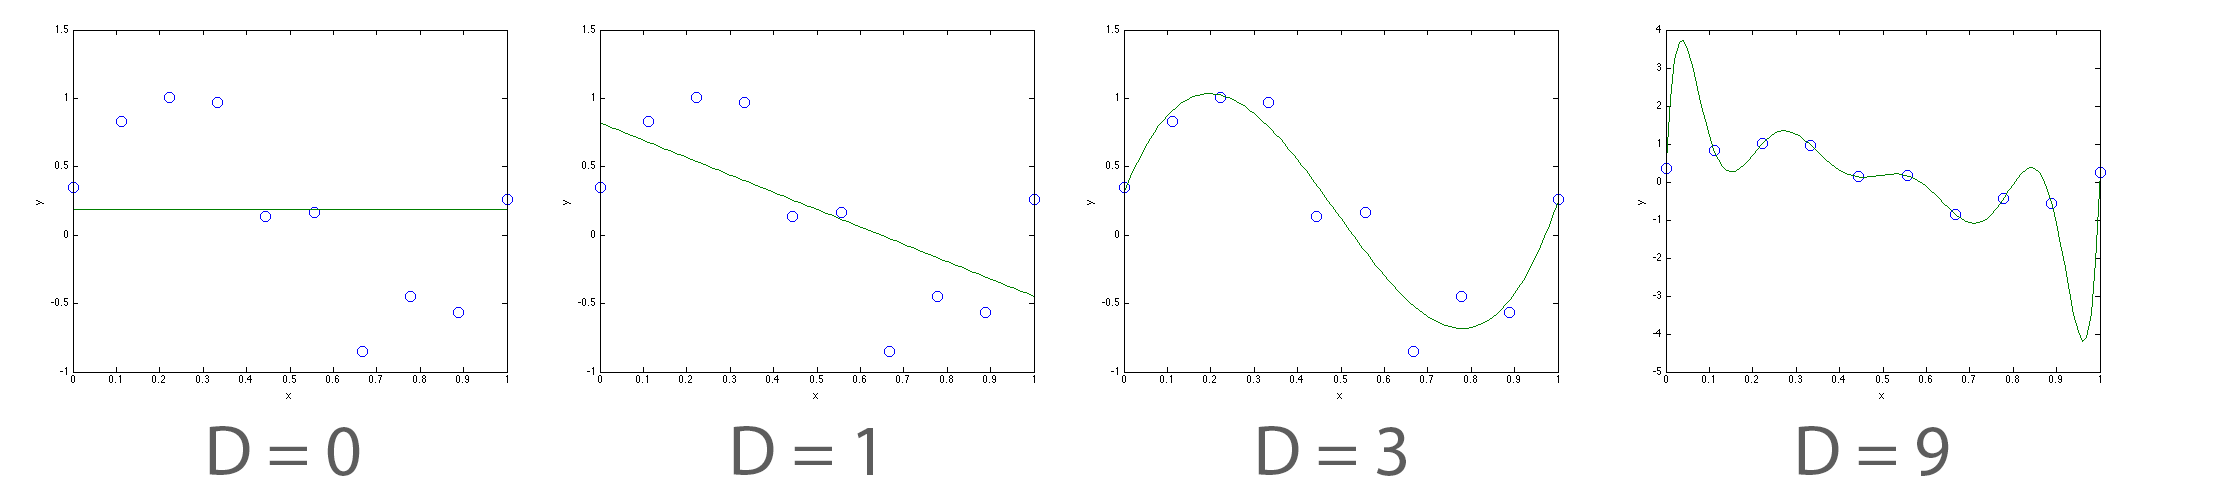
\includegraphics[width=1.0\textwidth]{figures/problem_2_1_full.png}
\end{figure}

\end{document}
